\chapter{Project Management}
\label{chap:project-management}
\enlargethispage{4\baselineskip}

\section{Development Methodology}

Two choices shaped how this internship was run: Agile over a fixed
up-front specification, and Scrum over the other mainstream Agile
framework, Kanban.

\subsection{Why Agile}

The project's requirements were expected to sharpen as real company data
(historical staffing decisions, a wider variety of TDRs) arrived during
the internship, leaving no room to absorb a wrong up-front decision
discovered late. An Agile approach, short iterations, a working
increment each cycle, room to re-prioritize on what was actually
learned, fit this far better than one up-front specification followed by
a single final delivery.

\subsection{Why Scrum}

Kanban's continuous-flow model (work pulled through WIP-limited columns,
no fixed iteration length, no built-in periodic ceremony) suits a team
absorbing unpredictable work indefinitely, not a one-month internship
with a hard deadline and a single stakeholder who needs a promised,
fixed rhythm to check in on. Scrum's time-boxed sprints give both a real
forcing function (each week's end, a story is either done and demoable
or visibly not) and a fixed Sprint Review slot the company supervisor
could plan around from day one, rather than an open-ended stream of ad
hoc check-ins.

\section{Scrum Framework}

Scrum was adapted, not diluted, for a solo developer: the same roles,
artifacts, and events below still exist, just held by fewer people.

\subsection{Roles}

For this internship, the intern acted as both Developer and Product
Owner (backlog prioritization, sprint goal definition), with the
company supervisor as final approver. [Company Supervisor] acted as the
primary stakeholder for Sprint Reviews.

\subsection{Artifacts and Events}

Table~\ref{tab:artifacts} lists the Scrum artifacts this internship used, adapted to a solo-developer cadence; Table~\ref{tab:events} lists the events.

\begin{table}[H]
  \centering
  \caption{Scrum artifacts used in this internship}
  \label{tab:artifacts}
  \begin{tabular}{@{}p{3.2cm}p{14.4cm}@{}}
    \toprule
    Product Backlog & The full list of prioritized stories across all four sprints (Section~\ref{sec:product-backlog}). \\
    Sprint Backlog & The subset of stories committed to for the current sprint, each with acceptance criteria. \\
    Increment & The working, demoable software produced at the end of each sprint (see each sprint chapter's Sprint Review section). \\
    \bottomrule
  \end{tabular}
\end{table}

\begin{table}[H]
  \centering
  \caption{Scrum events used in this internship}
  \label{tab:events}
  \begin{tabular}{@{}p{3.2cm}p{14.4cm}@{}}
    \toprule
    Sprint Planning & At the start of each one-week sprint: selecting and estimating that sprint's backlog. \\
    Daily tracking & A short daily log of progress and blockers, in place of a synchronous stand-up given the solo setup. \\
    Sprint Review & A demo of the sprint's working increment to the company supervisor. \\
    Sprint Retrospective & A short review of what worked and what to change for the next sprint. \\
    \bottomrule
  \end{tabular}
\end{table}

\section{Product Backlog}
\label{sec:product-backlog}

The full product backlog covers 33 stories across four sprints, organized
into seven epics: ingestion \& extraction, matching engine, anomaly
detection, reporting \& explainability, dashboard UX, DevOps, and company
profile, the last one kept in the \emph{icebox}, Scrum's term for ideas
explicitly parked and not scheduled into any of the four sprints, rather
than silently dropped. Story points follow a Fibonacci-like scale
(1, 2, 3, 5, 8); anything larger is split before being scheduled.

One deliberate structural decision shaped the whole plan: the
\texttt{dashboard-ux} epic is spread as a thin vertical slice across
every sprint rather than batched into the last one, so every Sprint
Review has a real, working screen to demo (upload/preview in Sprint 1,
matching results in Sprint 2, full report/review in Sprint 3) instead of
nothing showable until the very end.

\section{Sprint Planning}

Table~\ref{tab:sprint-plan} lays out the four sprints' dates, committed points, and demoable increment.

\begin{table}[H]
  \centering
  \caption{Four-sprint plan overview}
  \label{tab:sprint-plan}
  \begin{tabular}{@{}clrl@{}}
    \toprule
    Sprint & Dates & Points & Demoable increment \\
    \midrule
    1 & Jul 6 -- Jul 10  & 43 & Upload a real CV/TDR, see extracted structured fields \\
    2 & Jul 13 -- Jul 17 & 42 & Matching results page: ranked candidates, real scores \\
    3 & Jul 20 -- Jul 24 & 50 & Report view: rationale, citations, approve/reject/override \\
    4 & Jul 27 -- Jul 31 & 35 & Complete styled dashboard + metrics page with real numbers \\
    \bottomrule
  \end{tabular}
\end{table}

Sprint point totals were estimated to land reasonably close to each
other, though risk and complexity mattered more than exact parity:
Sprint 1 front-loads the riskiest technical
integration (multi-key LLM provider routing, since the project has no
paid API access) alongside project setup; Sprints 2 and 3 carry the core
pipeline complexity (retrieval, scoring, anomaly detection, report
generation); Sprint 4 winds down into polish and evaluation rigor.

\begin{figure}[H]
  \centering
  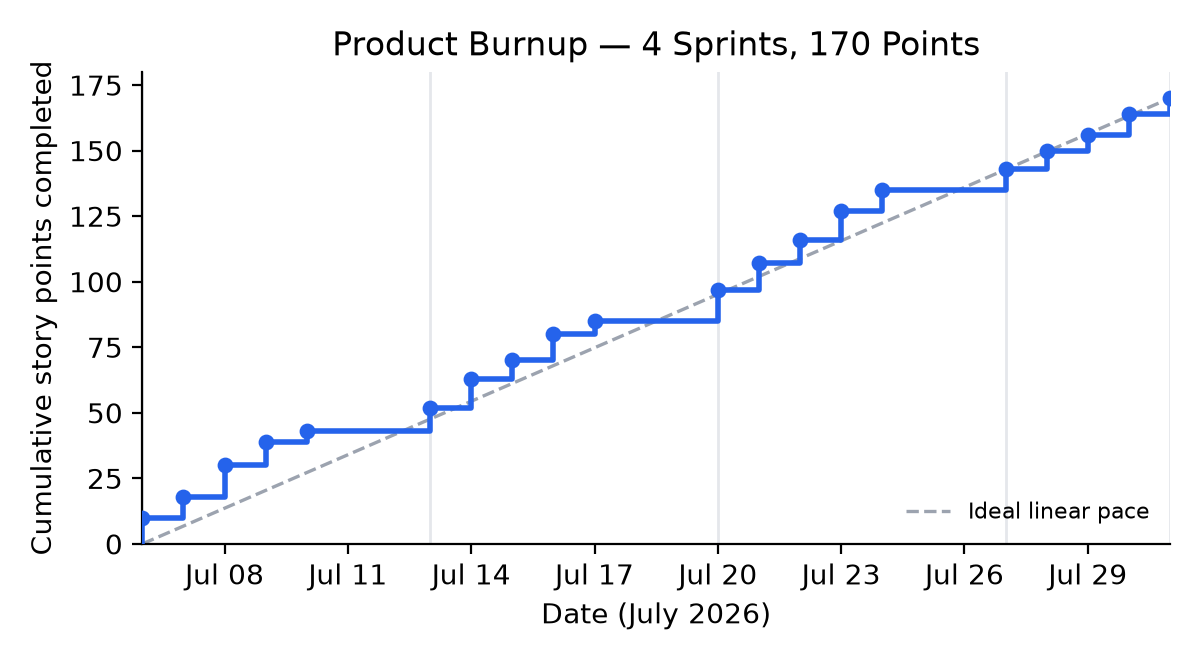
\includegraphics[width=0.48\textwidth]{burnup.png}
  \caption[Product burnup chart]{Product burnup chart: cumulative story points completed across
  the four sprints.}
  \label{fig:burnup}
\end{figure}

Points land day by day within each sprint's own window (implementation-
heavy early and mid-sprint, a lighter close-out day, flat weekends
between sprints), reaching all 170 points by July 31, Sprint 4's close;
the hardening work in Section~\ref{sec:post-sprint-hardening} happened
after, outside the four sprints' original scope.

\section{Development Environment}
\label{sec:dev-environment}
\enlargethispage{3\baselineskip}

This section covers the hardware, software stack, and version-control
and tracking practices used to build and ship AdéquIA.

\subsection{Hardware}

Development was carried out on a single development machine running
Windows, with Docker Desktop used to run PostgreSQL and Redis locally.

\subsection{Software \& Technologies}

Table~\ref{tab:tech-stack} summarizes the stack used across the backend, frontend, and CI/CD.

\begin{table}[H]
  \centering
  \caption{Technology stack}
  \label{tab:tech-stack}
  \begin{tabular}{@{}p{3.2cm}p{14.4cm}@{}}
    \toprule
    Backend & Python, FastAPI, LangGraph/LangChain, SQLAlchemy (async) with Alembic migrations, PostgreSQL with \texttt{pgvector}, Redis with RQ for background jobs. \\
    LLM providers & No paid API access: extraction/reasoning calls round-robin across free-tier Groq and Gemini key pools, falling back to a local Ollama model once every key is rate-limited. Embeddings run locally via \texttt{nomic-embed-text} (Ollama), with a later Gemini fallback for transient TDR-retrieval lookups (Section~\ref{sec:post-sprint-hardening}). \\
    Frontend & Next.js (App Router), TypeScript, Tailwind CSS, shadcn/ui (Radix primitives, Vega style preset). \\
    Testing \& quality & pytest, ruff, mypy (strict) on the backend; ESLint, TypeScript's compiler, and Next.js's build-time checks on the frontend. \\
    CI/CD & GitHub Actions: lint/type-check/unit tests on every pull request, Docker image builds on merge to main, a manually-triggered RAGAS/DeepEval evaluation workflow. \\
    \bottomrule
  \end{tabular}
\end{table}

\subsection{Git Strategy}

Figure~\ref{fig:git-strategy} shows the branch lineage, each sprint cut
from the last rather than restarted from \texttt{master}, continued by
post-close hardening (Section~\ref{sec:post-sprint-hardening}) after
Sprint 4's close. Conventional Commits (\texttt{feat:}, \texttt{fix:},
\texttt{chore:}, \texttt{docs:}, \texttt{test:}) became the commit
convention from \texttt{sprint-1} on, each story and fix its own commit.
The backlog and sprint plans were also mirrored into Jira for
day-to-day tracking outside this report.

\begin{figure}[H]
  \centering
  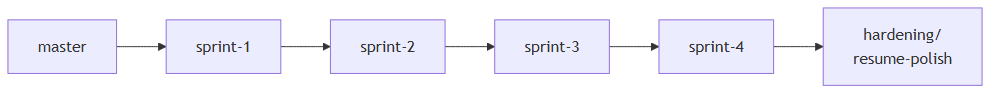
\includegraphics[width=0.85\textwidth]{s3-git-strategy.png}
  \caption[Git branch lineage]{Git branch lineage: each sprint branches from the last, not
  from \texttt{master}.}
  \label{fig:git-strategy}
\end{figure}
